\chapter{Architecture du projet}
\section{Relations}
    \subsection{Voisinages}
        Le voisinage d'un pièce correspond aux places du monde qui sont dirrectement en contact avec la place de la pièce. Le nombre de voisins d'une pièce dépend donc de la géométrie de notre plateau (cf. \textbf{\ref{part:geometry}}). On va déterminer ces derniers en testant l'entièreter des directions disponibles pour la pièce en omettant pas de verifier si les cases sont occupées ou non. Cela nous donne donc un ensemble de case disponible pour cette dernière qui repond bien aux contrainte géométrique du plateau.
    \subsection{Déplacements}
        Nos déplacements sont réalisés en modifiant dans le monde l'état de la position ainsi que l'index associé à la pièce en question. Cela informe donc aux autres pièces que cette position est prise et permets de savoir à quel joueur elle appartient.\\
        Pour determiner la position exacte du déplacement, on utilise un fonctionement de recherche de proche en proche, qui va déterminer les voisins direct, puis en fonction du nombre de mouvements de la pièce, rééfectuer ce processur avec le voisin direct situé de la direction souhaitée. Le déplacement de cette dernière se fait ensuite aléatoirement parmis ces possibilités et comme dit précédement, il est impossible pour cette dernière de choisir une case déja occupée. \\
        Dans le cas ou toutes les cases sont occupées le joueur ne peut pas jouer et sont tour est passé.
        
    \subsection{Chagements de terrain}
        Dès lors que la partie commence, une initialisation de la \textit{seed} du terrain est nécessaire. \\
        Cette \textit{seed} influe directement sur les intéractions entre les différente position du monde et change donc les déplacements possibles. Chaque pièce sera donc restraintes à un certain nombre de relations : \\
        
        \begin{itemize}
            \item Pour un terrain classique (hexagonal), toutes les direction sont autorisées.\\
            \item Pour un terrain à pavage triangulaire, une case sur deux possède les même relations de voisinage, on a ici les relations (N,SE,SW) pour une partie des pièces et (S,NE,NW) pour l'autre. \\
            \item Pour un terrain a pavage carré, les seuls directions autorisés sont celle des points cardinaux (N,S,E,W). \\ 
        \end{itemize}
        
        Après avoir réduit le nombre de directions possibles, le système de déplacement est appliqué de manière identique, elle prend alors compte des contraintes de directions. \\
        Nous avons donc réussis à implémenter un système qui en modifiant une \textit{seed} de terrain, modifie les relations de voisinage de la partie en cours.  
    \subsection{Positions de départ}
    En prenant en considération l'aspect torique de notre plateau nous avons souhaité le moins de déséquilibre possible au début de la partie. \\
    C'est pourquoi La position des pièces est choisie par le programme. Pour celà nous avons implémenté un algorithme qui, en fonction du nombre de pièces spéciales à placer, choisis une formation qui soit identique pour chaque joueur et qui ne crée pas de déséquilibre entre les joueurs, et ceci quelque soit le nombre de joueur. \\
            La figure \textbf{\ref{fig:depart_classique_a_4}} montre les positions de départ pour une partie lancée avec 4 joueurs, sur un monde de taille $10\times10$, avec  $2$ tours (pièce, cf. \textbf{\ref{part:tower}}) par joueurs.
            
            \begin{figure}[H]
                \centering
                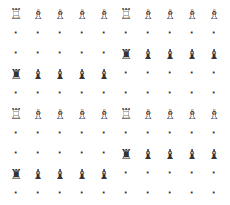
\includegraphics[scale=0.6]{img/depart_classique_a_4.png}
                \caption{Départ classique à 4}
                \label{fig:depart_classique_a_4}
            \end{figure}

        Cette facon de penser le départ du jeu nous a permis de rendre le jeu encore plus modulable et de l'adapter à beaucoup plus de configurations que ce qui nous était demandé avec des possibilité de départ presque infinie.
            
    \subsection{Capture et libération}
        Si une pièce atterit sur une pièce adverse, une capture est réalisée. Si la position de la pièce capturée est libre, elle a une probabilité d'être libérée. Cette probabilitée est fixé à \texttt{50/100} mais peut être modifié par l'utilisateur).
        La question de la capture d'une pièce adverse par un joueur est un des raisons qui nous ont poussé à créer un "monde extérieur" \texttt{world\_ext.c} (\textbf{cf. \ref{part:graph_src}}), qui sous forme d'une structre contient le plateau, les joueurs et les pions. \\

        \begin{Code}
            \begin{lstlisting}
struct world_ext_t {
	struct world_t* world;                         // Plateau de jeu
	int nb_players;                                // Nombre de joueurs.
	struct players_t players[WORLD_SIZE];          // Liste des joueurs.
	struct sets_t initial_sets[WORLD_SIZE];        // Ensembles de positions de départ des joueurs.
	struct sets_t current_sets[WORLD_SIZE];        // Ensembles de positions prises par chaque joueurs.
	int nb_captured_pawns;                         // Nombre de pièces capturées.
	struct pawns_t* captured_pawns[WORLD_SIZE];    // Liste des pièces capturées.
};\end{lstlisting} \end{Code}
        \noindent L'implémentation de cette fonction nous a permis d'implémenter la capture de cette façon : \\
        \begin{itemize}
            \item Lorsqu'une pièce est capturée, sont attribut \texttt{captured} (cf. \textbf{\ref{part:pawns}}) prend la valeur \texttt{1}.
            \item La pièce est ajoutée à la liste des pièces capturés : \texttt{captured\_pawns[]}, et sa position est retirée de la liste des positions prises par le joueur : \texttt{current\_sets[index\_du\_joueur][]}.
        \end{itemize} 

        \noindent \\ Procéder de cette manière nous a permis de ne pas modifier la position de la pièce capturée, ainsi, elle la garde en mémoire. Lorsque les conditions de libérations sont remplies, ont effectue le shéma inverse, et la pièce est de retour sur le plateau. 

\section{Inclusions et organisation du projet (Makefile?)}

    \subsection{Organisation du monde}
    \subsection{Dépendances des fichiers}\label{part:graph_src}
        Afin de rendre le projet le plus modulable possible, nous avons séparé notre projet en plusieurs fichiers \texttt{.c}, ces fichiers contienent les fonctions qui permettent au tout de fonctionner. Chacun de ces fichiers \texttt{.c} incluent un fichier \texttt{.h} du même nom. Ces fichiers d'entête contiennent les \texttt{header} de toutes les fonctions "publiques" qui ont pour but d'être utilisés par d'autre fichiers. Les inclusions ne se font jamais entre les fichier \texttt{.c}, mais uniquement avec les \texttt{.h}.
        
        \begin{figure}[H]
            \centering
            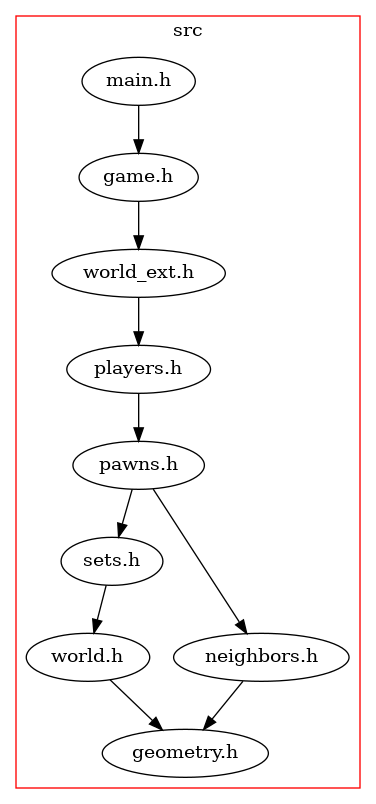
\includegraphics[scale=0.4]{img/graph_src.png}
            \caption{Graphique de dépendance des fichiers source. \textit{Généré avec} \texttt{Graphviz}.}
            \label{fig:graph_src}
        \end{figure}

        Cette organisation du projet à base d'inclusion nous permet une très grande modularité. En effet, si un fichier \texttt{.c} est modifié (comme par exemple \texttt{world.c}), le projet continue de fonctionner tant que la nouvelle implémentation respecte le fichier \texttt{.h} correspondant.

    \subsection{Compilation}
        Pour faciliter les travaux de compilations séparés, nous avons intégrés un fichier \texttt{Makefile}. Ce fichier nous a permis de déclarer des règles générales qui simplifient les commandes de compilations. Nous nous en somme par exemple servis pour compiler automatiquement tout les fichiers \texttt{.o} nécessaire, ou encore pour compiler et éxécuter tout les tests en même temps.

\section{Tests}
    \subsection{Structure des tests}
        Nous avons décidés de séparer les tests dans différentes fichier pour plus de flexibilité. Chaque fichier test contient les fonctions visants à tester un unique fichier source. Cette méthode nous à permis de pouvoir tester l'ensemble du code source en même temps, ou bien de lancer les tests d'un fichier en particulier. \\

        \begin{figure}[H]
            \centering
            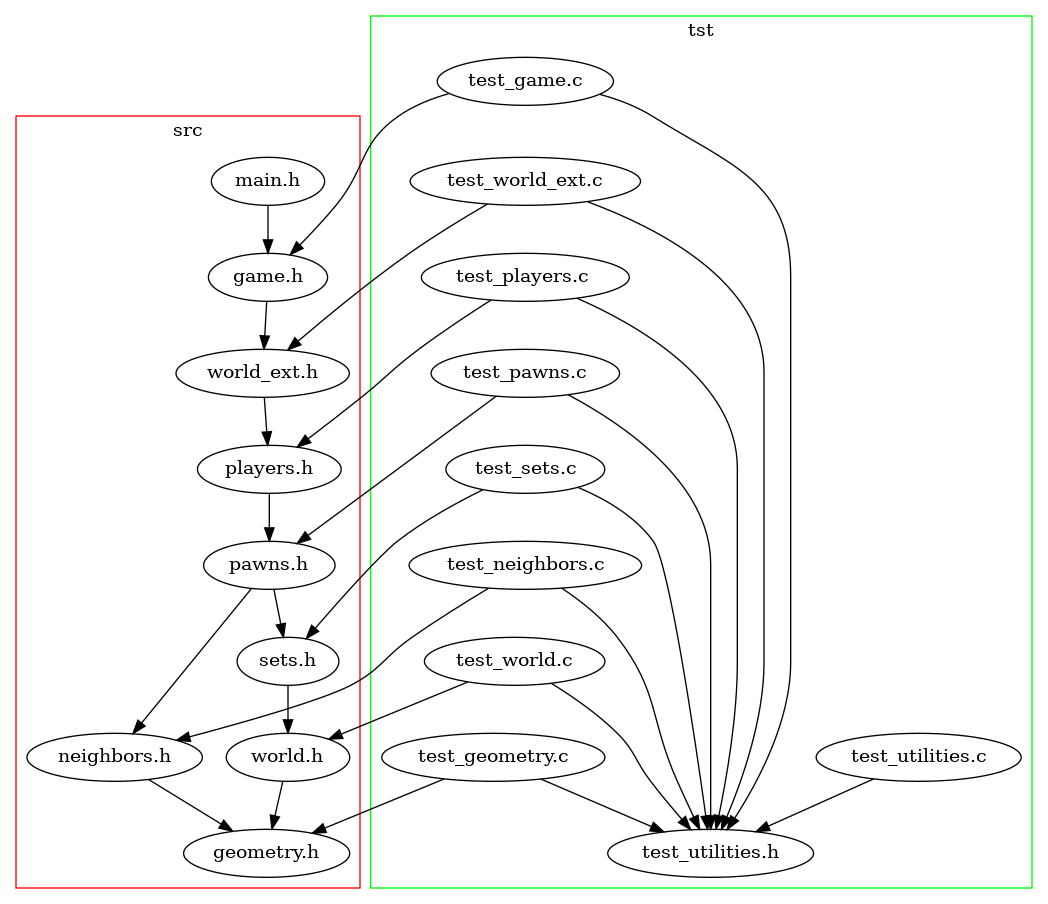
\includegraphics[scale=0.4]{img/graph_tst.png}
            \caption{Graphique de dépendance des fichiers tests. \textit{Généré avec} \texttt{Graphviz}.}
            \label{fig:graph_tst}
        \end{figure}

        La figure \textbf{\ref{fig:graph_tst}} montre les inclusions de nos fichiers test. On remarque que chaque fichier test inclu uniquement le fichier source qu'il teste. \\
        
        De plus, nous avons décidés de séparer deux fonctions générales des tests dans un fichier \texttt{test\_utilities.c}. Ce fichier est le seul des fichiers tests à avoir un fichier d'entête, car c'est le seul qui est inclu dans d'autres fichiers. Il contient les deux fonctions suivantes :

        \begin{Code}
            \begin{lstlisting}
void str_test(const char str1[], const char str2[]) // Compare 2 strings
{ 
    (!strcmp(str1, str2)) ? printf("\t\tPASSED\n") : printf("\t\tRecieve %s instead of %s.\n", str1, str2);
}

void int_test(const int int1, const int int2) // Compare 2 integers
{
    (int1 == int2) ? printf("\t\tPASSED\n") : printf("\t\tRecieve %d instead of %d.\n", int1, int2);
}\end{lstlisting}
        \end{Code}

        C'est deux fonctions nous ont étés très utiles dans le cadre de la \textbf{programmation par le test}. En effet, appeller celles-ci dans nos fichier test nous a permis de très facilement comparés les retours des fonctions testés avec ce que nous attendions. En cas de réussite, le programme affiche : \texttt{PASSED}, tandis que si le test ne passe pas, le programme affichera : \texttt{Recieve <valeur\_reçu> instead of <valeur\_attendue>}.

        Nous avons donc pu écrire nos tests, puis implémenter nos fonctions jusqu'à ce que tout nos test affiches : \texttt{PASSED}.
        
    \subsection{Programmation par le test}
